\section{Results}
\label{sec:results}

In order to test and compare the methods presented in \cref{sec:proposed-method},
the methods were applied to real PV time series data, described in detail in \cref{sec:data-source}.
The results shown in this section are for the PV time series covering
926 days from 31 March, 2021 to 30 September, 2023.

\subsection{Day-ahead forecasts}

Using data available prior to sunrise, the proposed day-ahead forecast method from  \cref{sec:method-day-ahead} was applied to each of the weather forecast sources
(MGM meteogram cloudiness, SolCast cloudiness, and SolCast ghi)
to forecast the upcoming one-day (24 hr) PV output.
Following findings from \cite{Almeida2015},
28 days of historical data was used to fit the regression models.
An example day-ahead forecast using the Solcast GHI forecast is shown in \cref{fig:dayahead-forecast-solcast}. %

% /results/dayahead_method_comparison/SolCastGHIForecasts.pdf  page 27, with margins cropped
\begin{figure}[!ht]
	\centering
	% trim=left botm right top
	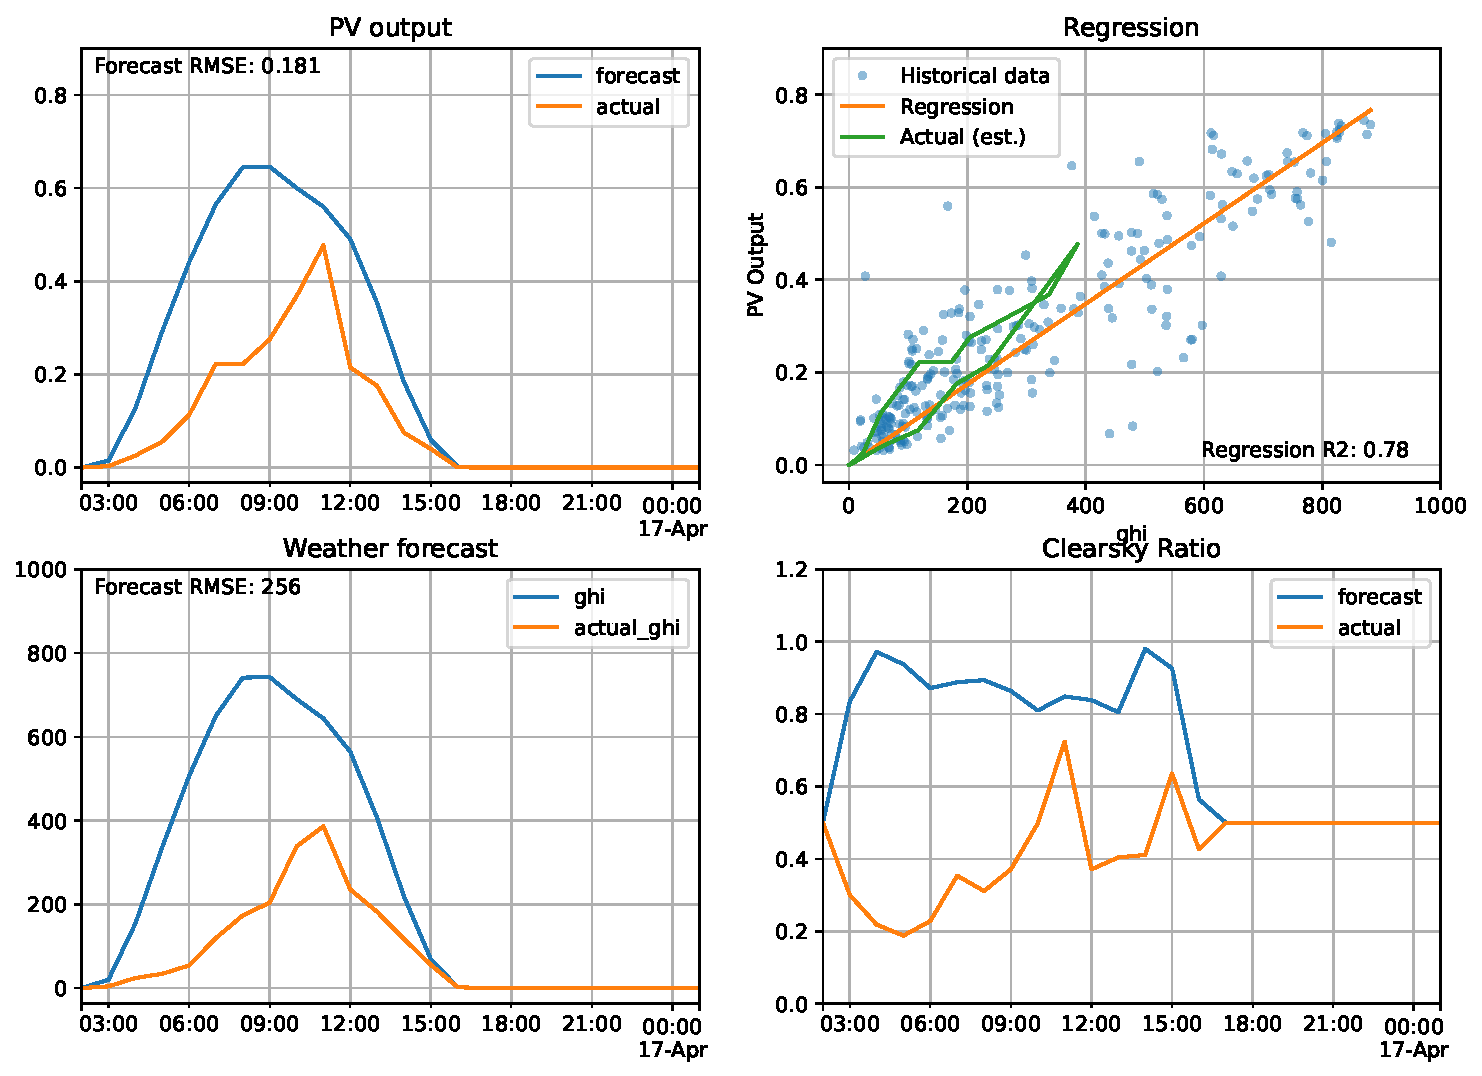
\includegraphics[width=1.0\columnwidth]{SolCastGHIForecasts-p27-cropped.pdf}
	% Convert to png: pdftoppm SolCastForecasts_w_regr_out_p41.pdf SolCastForecasts_w_regr_out_p41 -singlefile -cropbox -png -r 1200
	%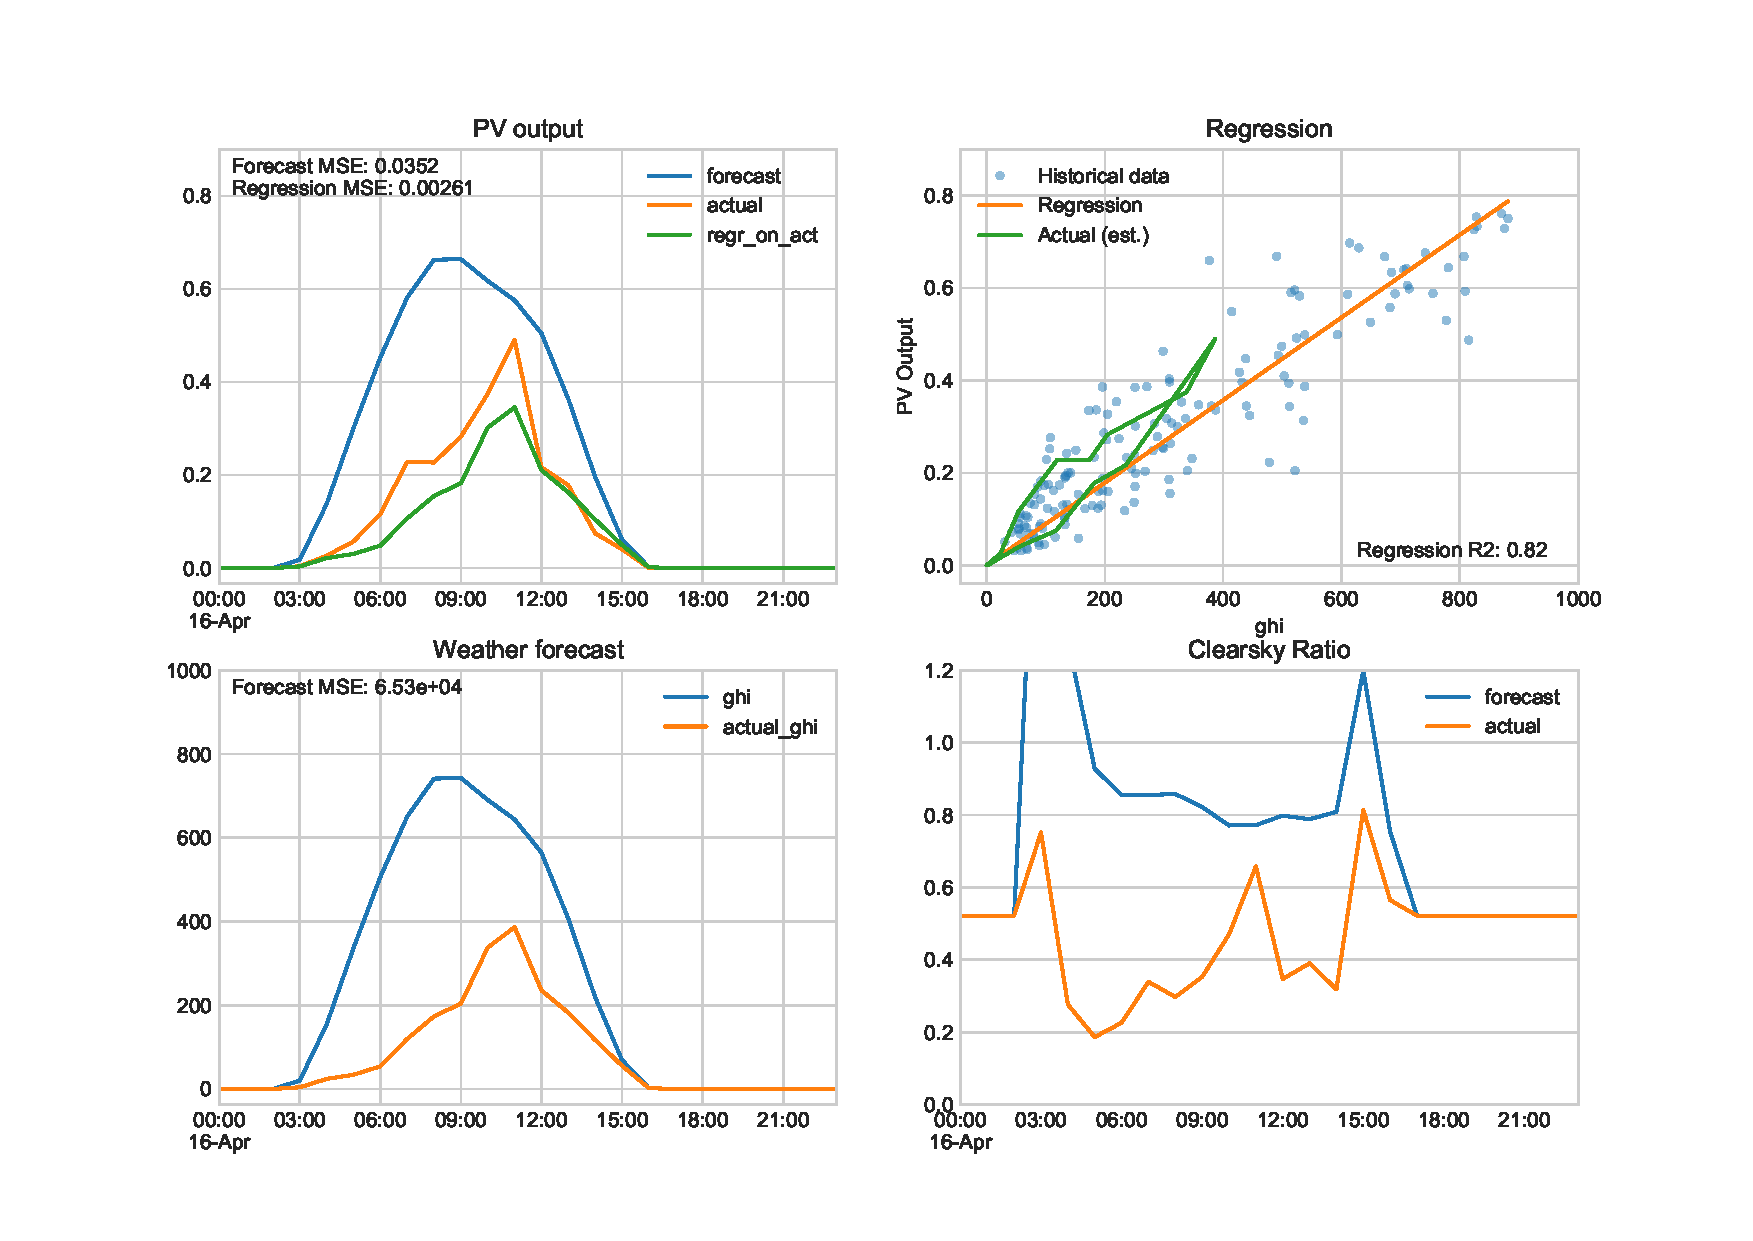
\includegraphics[width=6.5in]{SolCastForecasts_w_regr_out_p41.png}
	\caption{Example Day-ahead Forecast using Solcast GHI Forecast}
	\label{fig:dayahead-forecast-solcast}
\end{figure}

In addition to the proposed method, a reference day-ahead persistence forecast was also generated.
The persistence forecast was that the PV output for the upcoming period will be the same as the PV output for the same time of day in the previous day.

Following \cite{Pedro2012} and \cite{Gigoni2018}, the methods were evaluated using root mean square error (RMSE), mean absolute error (MAE), and mean bias error (MBE) as the error measure.
These metrics were calculated for of the whole time series as well as the for the forecast total energy output for each day.
The resulting error metrics are shown in \cref{table:dayahead-metrics} and \cref{table:dayahead-metrics-sum} respectively.

% Data for this table is from the file
% /results/dayahead_method_comparison/error_comparison_table.tex
\begin{table}[!t]
	\centering
	\caption{Day-ahead forecast metrics\pdfcomment[color=yellow]{Updated numbers in Tables 1, 2, and 3 for expanded time range}}
	\label{table:dayahead-metrics}
	\sisetup{round-mode=places,
		     round-precision=3}
	\begin{tabular}{lS[table-format=1.3]S[table-format=1.3]>{\sisetup{round-precision=4}}S[table-format=-1.4]}
		\toprule
		                       &   {RMSE}   &   {MAE}    &    {MBE}    \\
        \midrule
		Persistence & 0.108008 & 0.045457 & -0.000056 \\
		SolCast Cloudiness & 0.079121 & 0.036570 & -0.005733 \\
		SolCast GHI & 0.080192 & 0.036055 & -0.005092 \\
		MGM Meteogram & 0.088710 & 0.043129 & -0.007566 \\
		\bottomrule
	\end{tabular}
\end{table}

\Cref{fig:error-comparison-rmse-by-month} \pdfmarkupcomment[color=yellow]{shows the RMSE of the day-ahead forecasts when broken down by month of the year. The generally predictable climate pattern of clear summer skies is evident in the higher accuracy of all forecasting methods in the summer months of July and August.}{Added  figure and discussion in response to reviewers who wanted to know how the methods perform in different seasons.}

% This figure is from the file
% /results/dayahead_method_comparison/error_comparison_rmse_by_month.pdf  No post-processing used
\begin{figure}[tbh]
	\centering
	% trim=left botm right top
	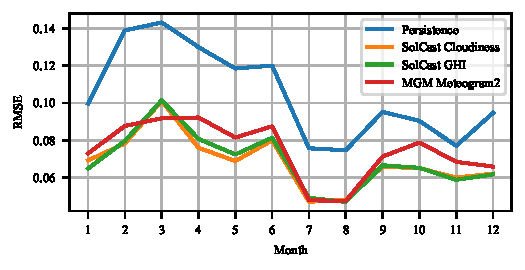
\includegraphics[width=1.0\columnwidth]{error_comparison_rmse_by_month.pdf}
	%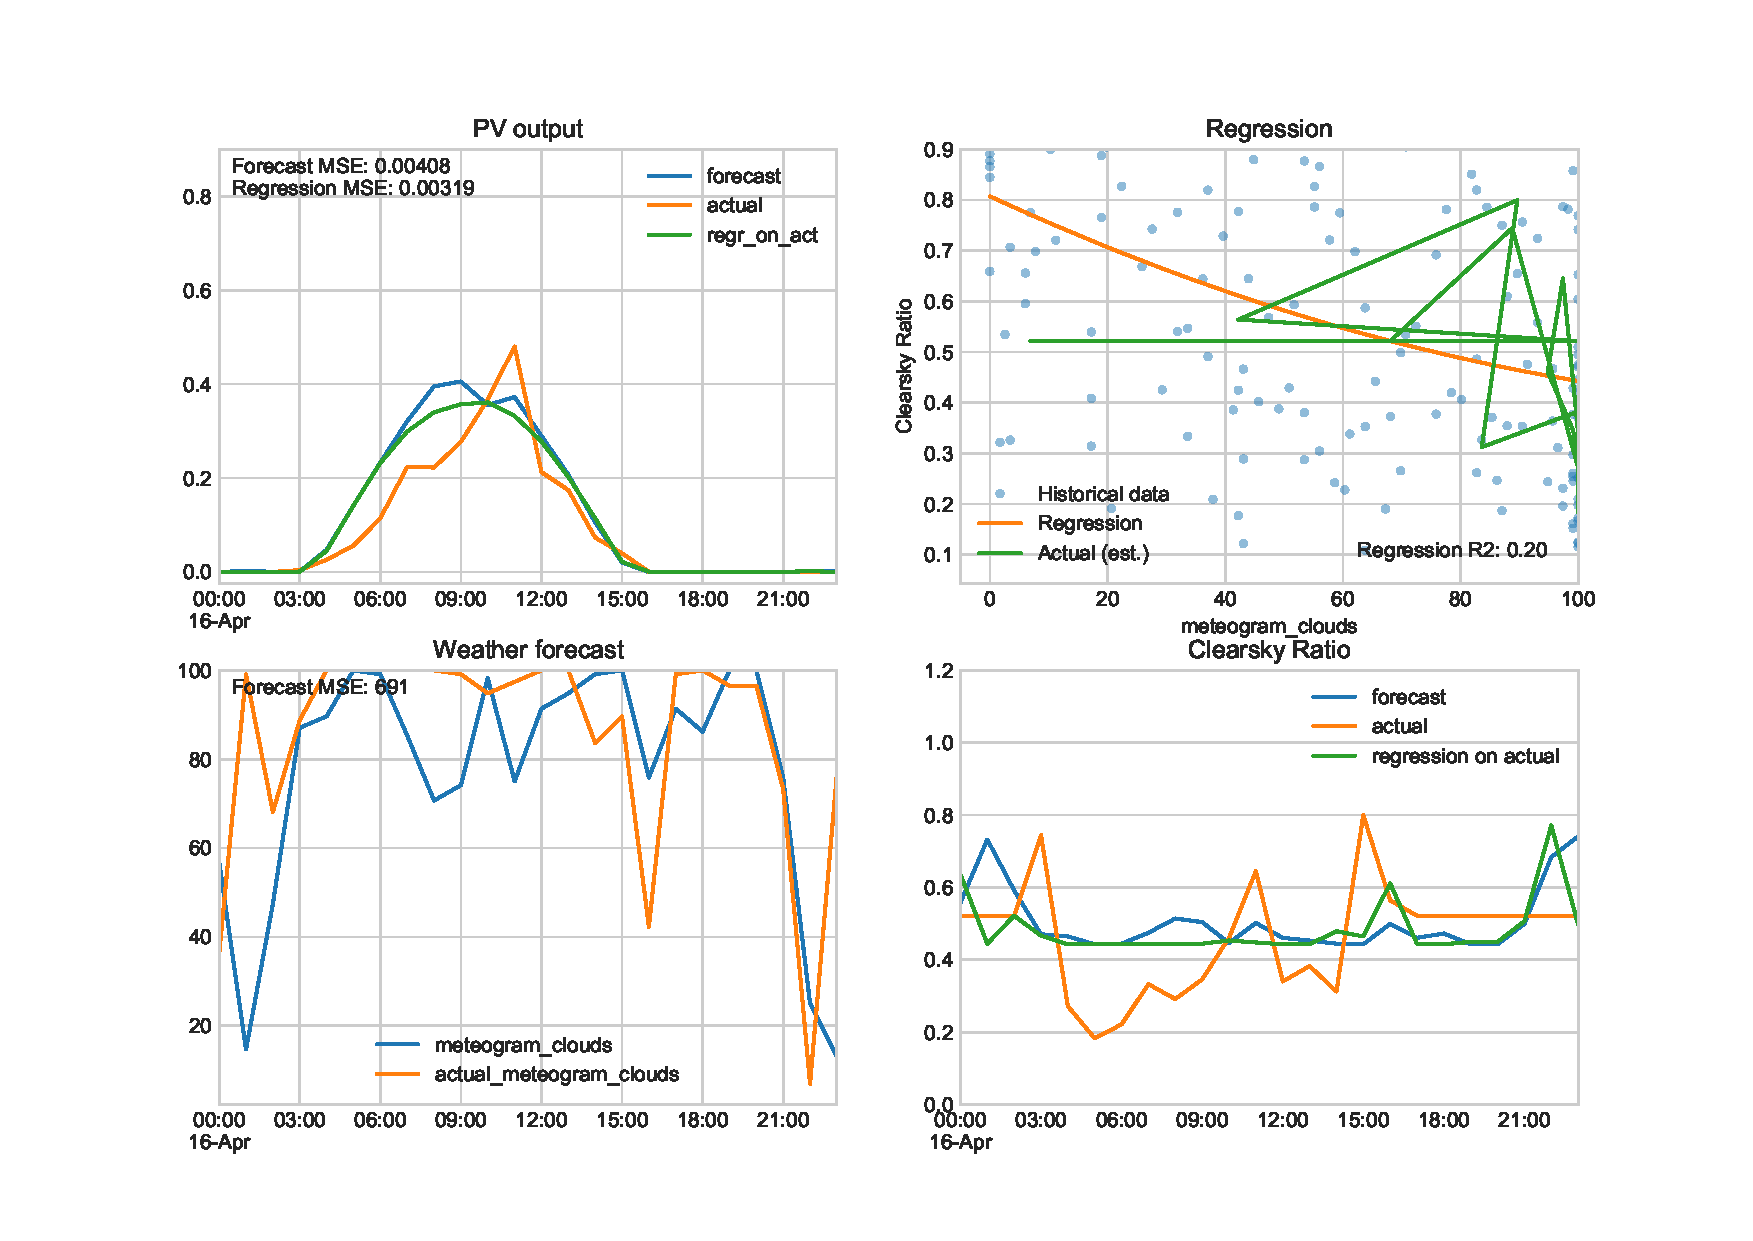
\includegraphics[width=6.5in]{MeteogramForecasts_cs_ratio_p41.png}
	\caption{Day-ahead Forecast RMSE by Month}
	\label{fig:error-comparison-rmse-by-month}
\end{figure}

% Data for this table is from the file
% /results/dayahead_method_comparison/error_comparison_table_daily_total.tex
\begin{table}[!t]
	\centering
	\caption{Day-ahead forecast metrics on daily sums}
	\label{table:dayahead-metrics-sum}
	\sisetup{round-mode=places,
		round-precision=3}
	\begin{tabular}{lS[table-format=1.3]S[table-format=1.3]S[table-format=-1.3]}
		\toprule
		                       &   {RMSE}   &   {MAE}    &    {MBE}    \\
        \midrule
		Persistence & 1.261943 & 0.873835 & -0.001353 \\
		SolCast Cloudiness & 0.917348 & 0.570336 & -0.137452 \\
		SolCast GHI & 0.911198 & 0.576658 & -0.122080 \\
		MGM Meteogram & 0.934198 & 0.557860 & -0.136774 \\
		\bottomrule
	\end{tabular}
\end{table}


\subsection{Intra-day Updates}

To evaluate and compare the intra-day forecast update methods,
as a starting point, a day-ahead forecast was first generated using the
SolCast cloudiness forecast.
This day-ahead forecast was then updated for each hour of the day using each of the methods proposed in \cref{sec:method-intraday}.
In addition to the proposed methods, a reference intra-day update forecast based on persistence was produced.
The persistence forecast was that the clear-sky ratio for the remainder of the day would be the same as the clear-sky ratio from the previous time period.

For comparison, the RMSE, MAE, and MBE for the different intra-day forecast update methods were computed
for the forecast for the periods 0 to 1, 1 to 2, and 6 to 7 hours after of the time at which the forecast is generated.
The resulting error metrics are shown in \cref{table:intraday-metrics}.
Note that the intra-day forecast metrics exclude nighttime hours since intra-day updates are not applied to them.

% Table data from
% /results/intraday_method_comparison/error_comparison_table.tex
\begin{table}[tb]
	\centering
\begin{threeparttable}
	\caption{Intraday forecast metrics}
	\label{table:intraday-metrics}
	\sisetup{round-mode=places,
		round-precision=4}
	\begin{tabular}{clS[table-format=1.4]S[table-format=1.4] >{\sisetup{round-precision=4}}S[table-format=-1.4]}
		\toprule
		\shortstack{Hours\\Ahead} & {Method} & {RMSE} & {MAE} & {MBE} \\
		\midrule
		\multirow[c]{6}{*}{0 - 1} & No update & 0.126005 & 0.094915 & -0.006438 \\
		& Persistence & 0.087132 & 0.057455 & -0.003383 \\
		& fx\_output\tnote{1} & 0.087592 & 0.062191 & -0.003949 \\
		% & fx\_csratio\tnote{2} & 0.086909 & 0.060625 & 0.000521 \\
		& exog\tnote{2} & 0.090861 & 0.068151 & 0.021551 \\
		& sarimax & 0.090069 & 0.064636 & 0.002129 \\
		& scaling & 0.091690 & 0.061761 & -0.000821 \\
		\midrule
		\multirow[c]{6}{*}{1 - 2} & No update & 0.123005 & 0.090430 & -0.004166 \\
		& Persistence & 0.110134 & 0.072331 & -0.006418 \\
		& fx\_output\tnote{1} & 0.105942 & 0.076733 & -0.003053 \\
		% & fx\_csratio\tnote{2} & 0.104632 & 0.074071 & 0.001245 \\
		& exog\tnote{2} & 0.113910 & 0.088160 & 0.038186 \\
		& sarimax & 0.109042 & 0.080150 & 0.007030 \\
		& scaling & 0.112747 & 0.076054 & -0.002213 \\
		\midrule
		\multirow[c]{6}{*}{6 - 7} & No update & 0.067470 & 0.033187 & -0.006961 \\
		& Persistence & 0.080227 & 0.037925 & -0.012122 \\
		& fx\_output\tnote{1} & 0.068531 & 0.034695 & -0.007467 \\
		% & fx\_csratio\tnote{2} & 0.065369 & 0.031866 & -0.006138 \\
		& exog\tnote{2} & 0.075610 & 0.038661 & 0.016232 \\
		& sarimax & 0.069811 & 0.035670 & -0.002428 \\
		& scaling & 0.078117 & 0.036695 & -0.007487 \\
		\bottomrule
	\end{tabular}
	\begin{tablenotes}
		\footnotesize
		\item[1] AR(2) on residual of PV output.
		% \item[2] AR(2) on residual of clear-sky ratio
		\item[2] AR(2) on actual output with exogenous variable
	\end{tablenotes}
\end{threeparttable}
\end{table}

% Figure from
% /results/intraday_method_comparison/IntradayUpdate-sarimax.pdf, p4, cropped to top plot
\begin{figure}[tb]
	\centering
	% trim=left botm right top
	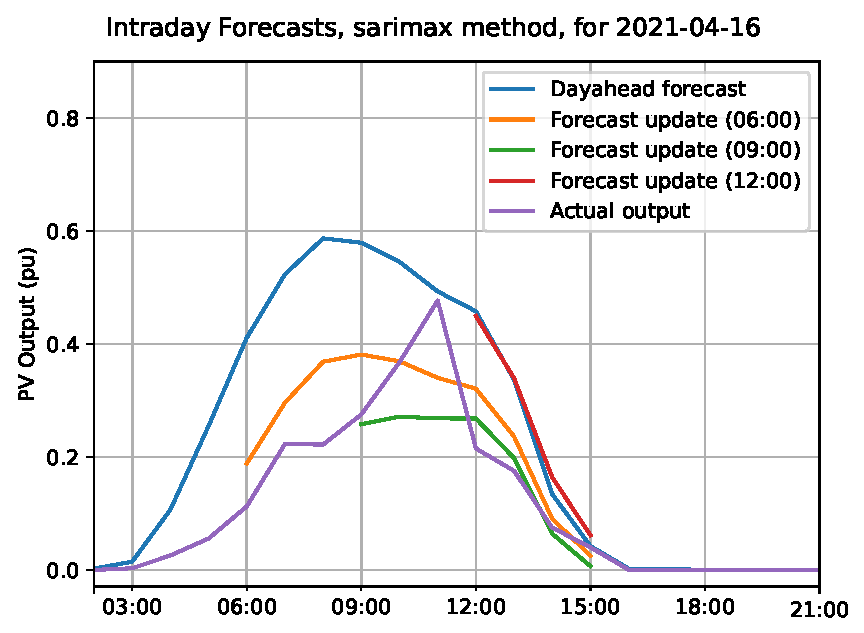
\includegraphics[width=0.85\columnwidth]{IntradayUpdate-sarimax-p4-cropped.pdf}
	%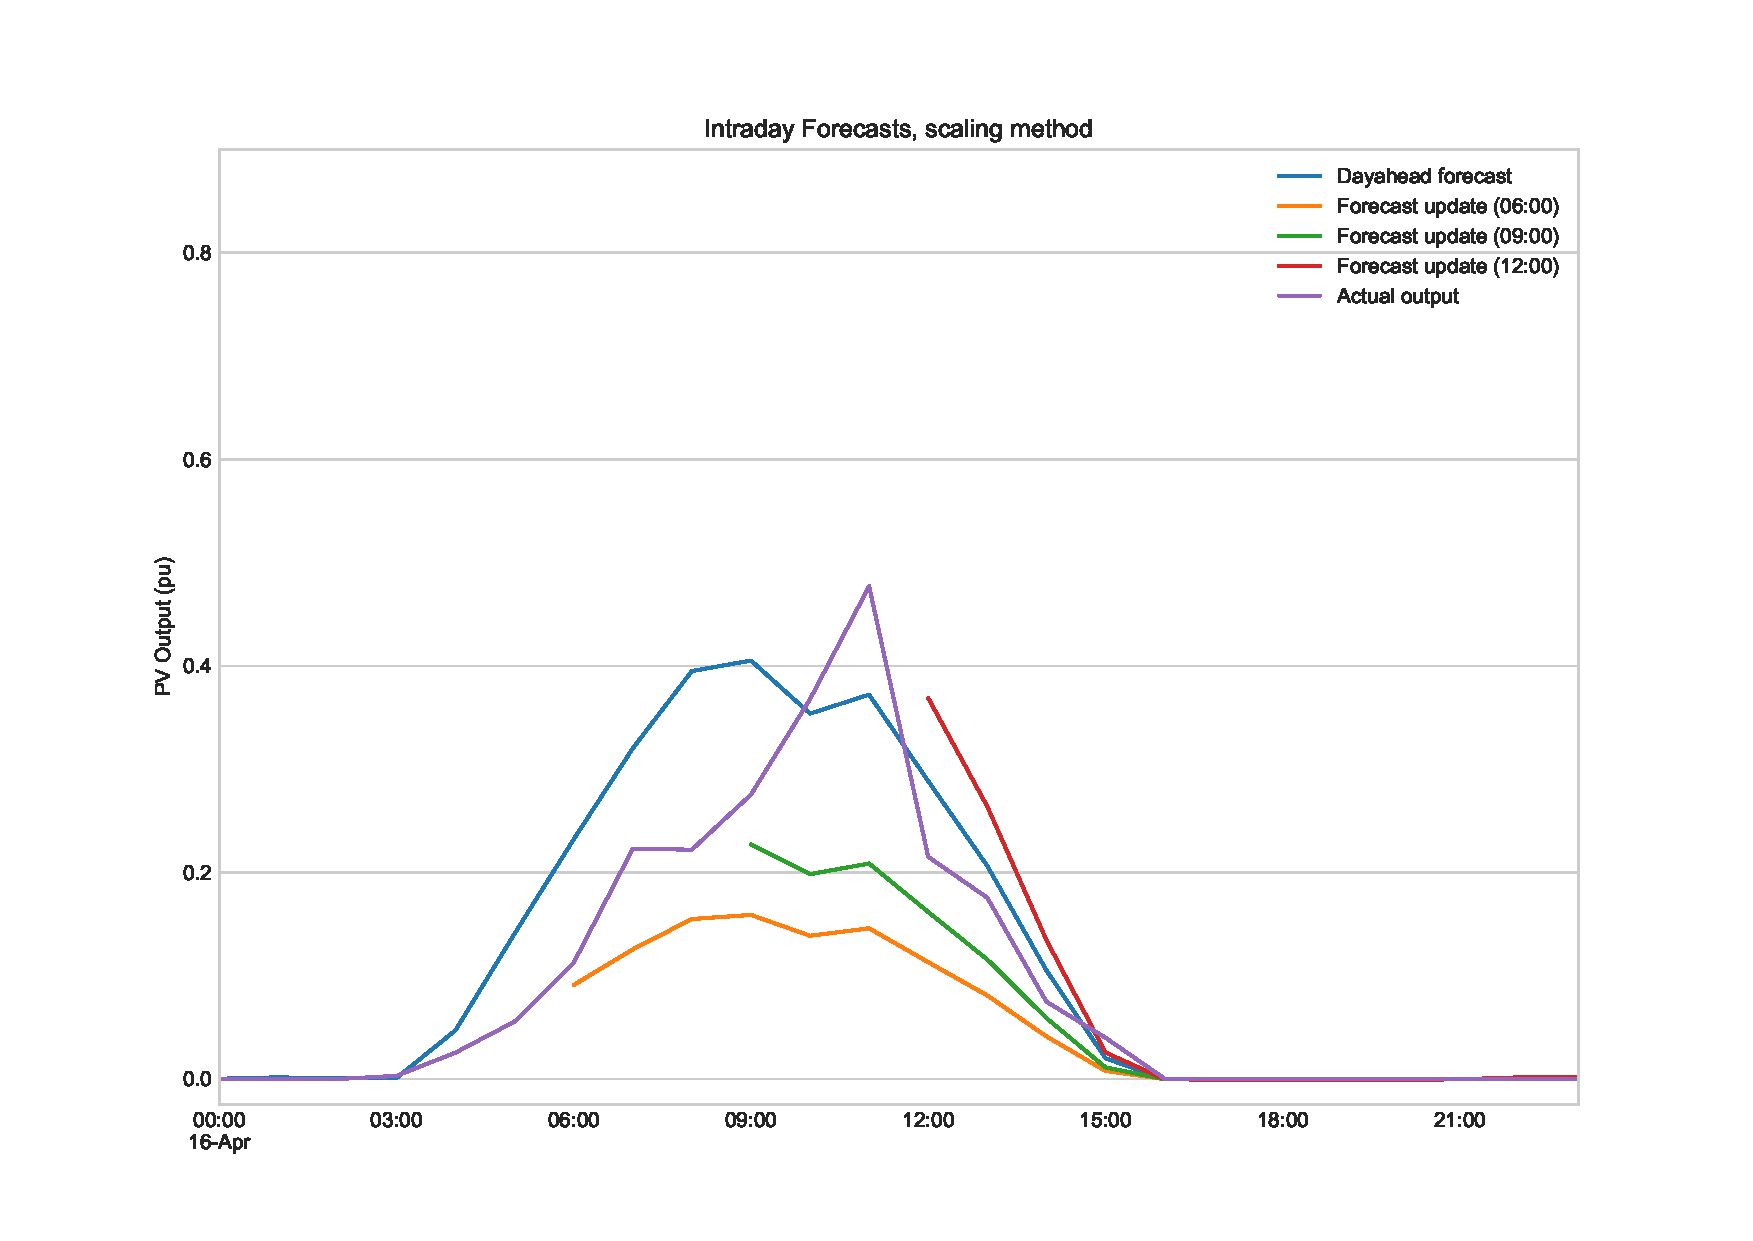
\includegraphics[width=5.53in]{Intraday Forecasts_p4.png}
	\caption{Intra-day Forecast Updates - SARIMAX method}
	\label{fig:intraday-forecast}
\end{figure}

% Discussion of benefits of intra-day updates
\pdfmarkupcomment[color=yellow]{
Comparison of the error metrics for the various intra-day update methods to the error metrics for the original dayahead forecasts shows that
the intra-day updates are most beneficial to the forecast accuracy in the upcoming few hours.
When considering six hours ahead, the weather-forecast-based day-ahead forecast tends to perform best without any proposed update methods.}{Added some discussion of the intra-day forecast results. I think the comparison to no update is helpful to see.}

\subsection{Optimal Energy Dispatch}

To demonstrate the effectiveness of the developed methods in the target application,
the forecasts were input into an agricultural microgrid operational optimization and simulation program.
A system diagram of the demonstration system is shown in \cref{fig:demo-system}.
The objective function for optimization is shown in \cref{eqn:objective-function}, where
$P_{grid,t}$ is the power drawn from the grid in each time period,
$P_{BSS,ch,t}$ and $P_{BSS,disch,t}$ are the battery system (BSS) charging and discharging powers,
$V_{use,desired,d}$ and $V_{use,d}$ are the desired and actual effective daily water use volumes,
$s_{BSS,t}$ is a binary variable representing the BSS charging mode, and
$s_{pump1,t}$ is a binary variable representing Pump 1 operating state.
$C_{grid,t}$, $C_{BSS}$, $C_{w,short}$, $C_{BSS,switching}$, and $C_{Pump1,switching}$ are the respective cost coefficients.
The optimization formulation was previously presented in full in \cite{Brown2022}.
%
\begin{equation}
	\label{eqn:objective-function}
	\begin{split}
		\min &\underbrace{\sum_t C_{grid,t} \ P_{grid,t} \ \Delta t}_{\textrm{Cost of grid power}}
		\\
		{+} \: &\underbrace{\sum_t C_{BSS} \left( P_{BSS,ch,t} + P_{BSS,disch,t} \right) \Delta t}_{\textrm{Cost of battery usage}}
		\\
		{+} \: &\underbrace{C_{w,short} \sum_d \max\left(\left(V_{use,desired,d} - V_{use,d}\right), 0\right)}_{\textrm{Penalty for inadequate water}}
		\\
		{+} \: &\underbrace{C_{BSS,switching} \sum_t \left| s_{BSS,t} - s_{BSS,t-1} \right|}_{\textrm{BSS mode-switching penalty}}
		\\
		{+} \: &\underbrace{C_{Pump1,switching} \sum_t \left| s_{pump1,t} - s_{pump1,t-1} \right|}_{\textrm{Pump 1 switching penalty}}
	\end{split}
\end{equation}


The use of model-predictive control (MPC) was simulated by using the optimizer to choose the optimal ratio of using excess available PV energy between energy storage in a battery energy storage system (BSS) and utilization to pump water into a reservoir.
The MPC optimization was performed using the forecast PV data, including intra-day updates.
The operation for the following period was then simulated using actual PV data.
A flowchart of the MPC simulation is shown in \cref{fig:mpc-simulation-flowchart}.

\begin{figure}[tb]
	\centering
	\fontsize{6pt}{7pt}\selectfont
	\def\svgwidth{0.8\columnwidth}
	\input{figs/demo_system.pdf_tex}
	\caption{Energy Dispatch Demonstration System}
	\label{fig:demo-system}
\end{figure}

\begin{figure}[tb]
	\centering
	% trim=left botm right top
	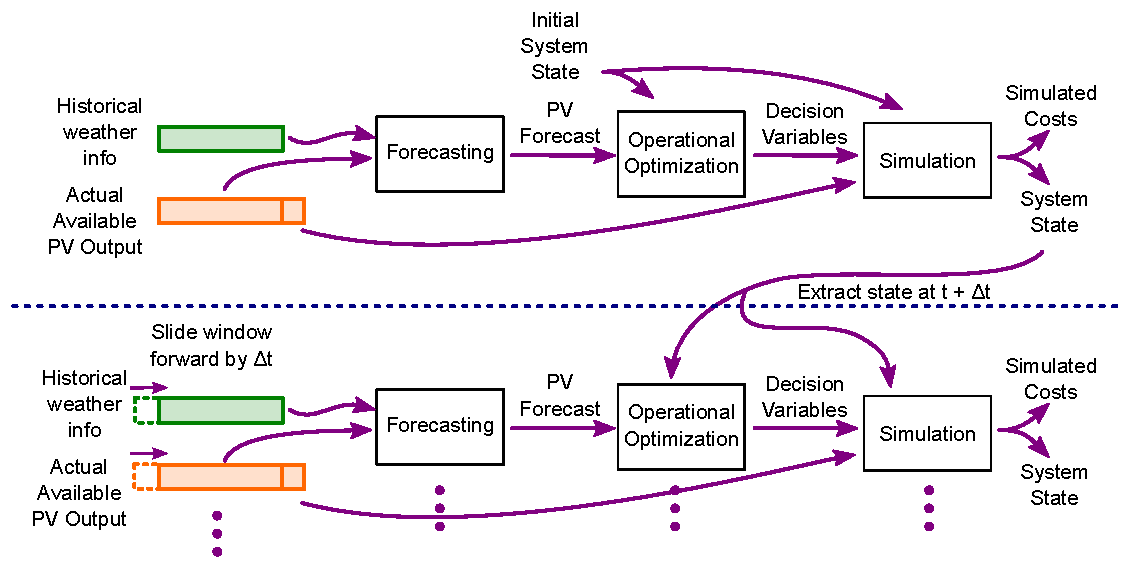
\includegraphics[width=1.0\columnwidth]{MPC Demo System Diagram.pdf}
	\caption{MPC demonstration simulation flowchart}
	\label{fig:mpc-simulation-flowchart}
\end{figure}

\pdfmarkupcomment[color=yellow]{The results shown in this section are for simulated operation for
64 days from 27 April to 29 June, 2021.}{Since this section's dates don't match the dayahead and intraday sections, they are now listed separately.} \Cref{table:mpc-simulation-results} shows results of the MPC simulation. Simulations were performed for three forecasts:

\begin{itemize}
\item Persistence forecast
\item SolCast cloudiness weather forecasts for day-ahead forecast with SARIMAX-based intraday updates
\item Perfect ``oracle'' forecast where operation is optimized with the actual future PV output data
\end{itemize}

The costs for the system's simulated operation using proposed forecast method was approximately
3\% lower than the performance using persistence forecasts.

The objective function value for optimized operation with a perfect forecast illustrates the value of improved forecasts.
An additional 8\% reduction in the objective function value would be possible with perfect forecasts.

% Data for this table is compiled from three different output files, one for each column
% Column 2 (Persistence forecast): /results/mpc_demo/seed=42,dayahead_method='persistence',intraday_method='persistence'/simulated_total_cost.tex
% Column 3 (Proposed method): /results/mpc_demo/seed=42,dayahead_method='solcast_clouds',intraday_method='sarimax'/simulated_total_cost.tex
% Column 4 (Perfect forecast): /results/mpc_demo/seed=42,dayahead_method='oracle',intraday_method='none'/simulated_total_cost.tex
% The data is manually entered into this file.
\begin{table}[!htb]
	\caption{MPC Simulation Results - Objective Function Value}
	\label{table:mpc-simulation-results}
	\centering
	\setlength\tabcolsep{0.6mm}
	\begin{tabular}{lS[table-format=5]S[table-format=5]S[table-format=5]}
		\toprule
		  Cost component
          & {\shortstack{Persistence\\Forecast}} & {\shortstack{Proposed\\Method}} & {\shortstack{Perfect\\Forecast}} \\
		  & {(\$, 2020)} & {(\$, 2020)}                    & {(\$, 2020)} \\
		\midrule
		Grid energy            & 65350 & 63764 & 58052 \\
		Battery use            &  8117 &  8178 &  8047 \\
		Inadequate water       &   865 &    71 &    10 \\
		Battery mode switching &   246 &   236 &   230 \\
		Pump switching         &    94 &    98 &    80 \\
		\midrule
		TOTAL                  & 74672 & 72347 & 66418 \\
		\bottomrule
	\end{tabular}
\end{table}

